% Convert with command:
% convert -density 300 pic.pdf -quality 90 pic.png
\documentclass[crop,tikz,border=0pt]{standalone}
\usetikzlibrary{arrows.meta, fit}
\begin{document}
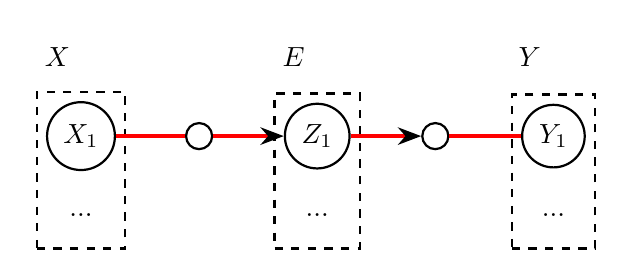
\begin{tikzpicture}

\begin{scope}[every node/.style={circle,thick,draw}]
    \node (x) at (0, 0) [shape=circle, fill=white] {$X_1$};
    \node (xs) at (0, -1) [shape=circle,draw=white] {...};
    \node (xtext) at (-0.3, 1) [shape=circle,draw=white,fill=white] {$X$};

    \node[draw,shape=rectangle,dashed,fit=(x) (xs)] {};

    \node (xz) at (1.5, 0) [shape=circle,draw=black] {};

    \node (z) at (3, 0) [shape=circle, fill=white] {$Z_1$};
    \node (zs) at (3, -1) [shape=circle,draw=white] {...};
    \node (ztext) at (2.7, 1) [shape=circle,draw=white,fill=white] {$E$};

    \node[draw,shape=rectangle,dashed,fit=(z) (zs)] {};

    \node (zy) at (4.5, 0) [shape=circle,draw=black] {};

    \node (y) at (6, 0) [shape=circle, fill=white] {$Y_1$};
    \node (ys) at (6, -1) [shape=circle,draw=white] {...};
    \node (ytext) at (5.7, 1) [shape=circle,draw=white,fill=white] {$Y$};

    \node[draw,shape=rectangle,dashed,fit=(y) (ys)] {};
\end{scope}

\begin{scope}[>={Stealth[black]},
            %   every node/.style={fill=white,rectangle,above},
              every edge/.style={draw=red,very thick}]

    \path [-] (x) edge node {} (xz);
    \path [->] (xz) edge node {} (z);

    \path [->] (z) edge node {} (zy);
    \path [-] (zy) edge node {} (y);
\end{scope}
\end{tikzpicture}

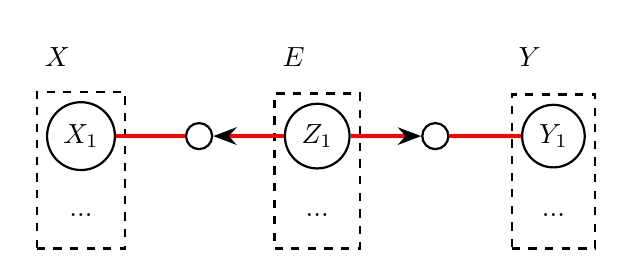
\begin{tikzpicture}

\begin{scope}[every node/.style={circle,thick,draw}]
    \node (x) at (0, 0) [shape=circle, fill=white] {$X_1$};
    \node (xs) at (0, -1) [shape=circle,draw=white] {...};
    \node (xtext) at (-0.3, 1) [shape=circle,draw=white,fill=white] {$X$};

    \node[draw,shape=rectangle,dashed,fit=(x) (xs)] {};

    \node (xz) at (1.5, 0) [shape=circle,draw=black] {};

    \node (z) at (3, 0) [shape=circle, fill=white] {$Z_1$};
    \node (zs) at (3, -1) [shape=circle,draw=white] {...};
    \node (ztext) at (2.7, 1) [shape=circle,draw=white,fill=white] {$E$};

    \node[draw,shape=rectangle,dashed,fit=(z) (zs)] {};

    \node (zy) at (4.5, 0) [shape=circle,draw=black] {};

    \node (y) at (6, 0) [shape=circle, fill=white] {$Y_1$};
    \node (ys) at (6, -1) [shape=circle,draw=white] {...};
    \node (ytext) at (5.7, 1) [shape=circle,draw=white,fill=white] {$Y$};

    \node[draw,shape=rectangle,dashed,fit=(y) (ys)] {};
\end{scope}

\begin{scope}[>={Stealth[black]},
            %   every node/.style={fill=white,rectangle,above},
              every edge/.style={draw=red,very thick}]

    \path [-] (x) edge node {} (xz);
    \path [<-] (xz) edge node {} (z);

    \path [->] (z) edge node {} (zy);
    \path [-] (zy) edge node {} (y);
\end{scope}
\end{tikzpicture}

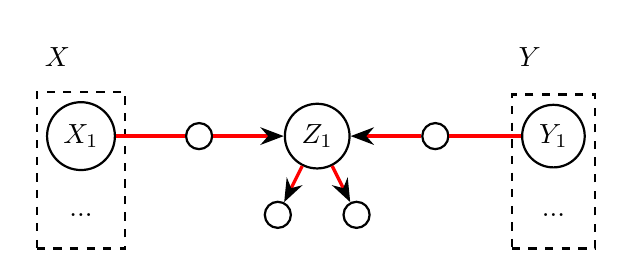
\begin{tikzpicture}

\begin{scope}[every node/.style={circle,thick,draw}]
    \node (x) at (0, 0) [shape=circle, fill=white] {$X_1$};
    \node (xs) at (0, -1) [shape=circle,draw=white] {...};
    \node (xtext) at (-0.3, 1) [shape=circle,draw=white,fill=white] {$X$};

    \node[draw,shape=rectangle,dashed,fit=(x) (xs)] {};

    \node (xz) at (1.5, 0) [shape=circle,draw=black] {};

    \node (z) at (3, 0) [shape=circle, fill=white] {$Z_1$};
    \node (z1) at (2.5, -1) [shape=circle,draw=black,fill=white] {};
    \node (z2) at (3.5, -1) [shape=circle,draw=black,fill=white] {};

    \node (zy) at (4.5, 0) [shape=circle,draw=black] {};

    \node (y) at (6, 0) [shape=circle, fill=white] {$Y_1$};
    \node (ys) at (6, -1) [shape=circle,draw=white] {...};
    \node (ytext) at (5.7, 1) [shape=circle,draw=white,fill=white] {$Y$};

    \node[draw,shape=rectangle,dashed,fit=(y) (ys)] {};
\end{scope}

\begin{scope}[>={Stealth[black]},
            %   every node/.style={fill=white,rectangle,above},
              every edge/.style={draw=red,very thick}]

    \path [-] (x) edge node {} (xz);
    \path [->] (xz) edge node {} (z);

    \path [<-] (z) edge node {} (zy);
    \path [-] (zy) edge node {} (y);

    \path [->] (z) edge node {} (z1);
    \path [->] (z) edge node {} (z2);
\end{scope}
\end{tikzpicture}

% Example
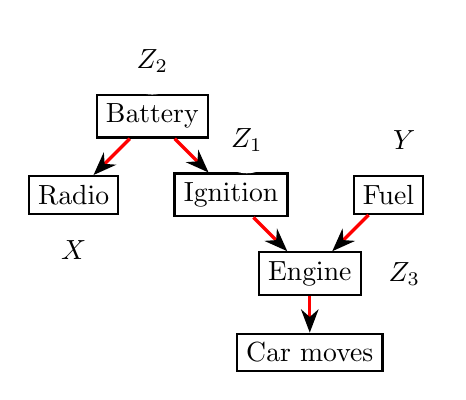
\begin{tikzpicture}

\begin{scope}[every node/.style={circle,thick,draw}]
    \node (battery) at (0, 0) [shape=rectangle, fill=white] {Battery};
    \node (z2) at (0, 0.7) [shape=circle,draw=white,fill=white] {$Z_2$};

    \node (radio) at (-1, -1) [shape=rectangle, fill=white] {Radio};
    \node (x) at (-1, -1.7) [shape=circle,draw=white,fill=white] {$X$};

    \node (ignition) at (1, -1) [shape=rectangle, fill=white] {Ignition};
    \node (z2) at (1.2, -0.3) [shape=circle,draw=white,fill=white] {$Z_1$};

    \node (fuel) at (3, -1) [shape=rectangle, fill=white] {Fuel};
    \node (y) at (3.2, -0.3) [shape=circle,draw=white,fill=white] {$Y$};

    \node (engine) at (2, -2) [shape=rectangle, fill=white] {Engine};
    \node (z3) at (3.2, -2) [shape=circle,draw=white,fill=white] {$Z_3$};

    \node (car-moves) at (2, -3) [shape=rectangle, fill=white] {Car moves};
\end{scope}

\begin{scope}[>={Stealth[black]},
            %   every node/.style={fill=white,rectangle,above},
              every edge/.style={draw=red,very thick}]
    \path [->] (battery) edge node {} (radio);
    \path [->] (battery) edge node {} (ignition);

    \path [->] (ignition) edge node {} (engine);
    \path [->] (fuel) edge node {} (engine);

    \path [->] (engine) edge node {} (car-moves);
\end{scope}
\end{tikzpicture}

\end{document}
